\documentclass[border={0pt 2pt 0pt 2pt}]{standalone}
\usepackage{amsmath,amssymb}
\usepackage{tikz}
\usetikzlibrary{arrows.meta,positioning,calc,bending}
% Shared, unscaled Springer artwork style. Compile from this directory.
\usepackage[T1]{fontenc}
\usepackage{amsmath,amssymb}
\usepackage{sansmathfonts}
\usepackage{tgheros}
\renewcommand{\familydefault}{\sfdefault}
\usepackage{sansmath}
% sansmath supplies Heros Latin letters; use sans fonts for Greek and symbols too.
\SetSymbolFont{letters}{sans}{OML}{cmssm}{m}{it}
\SetSymbolFont{symbols}{sans}{OMS}{cmsssy}{m}{n}
\SetSymbolFont{largesymbols}{sans}{OMX}{cmssex}{m}{n}
\usepackage{pgfplots}
\pgfplotsset{compat=1.18}
% Keep subscripts, superscripts and log tick exponents legible too.
\DeclareMathSizes{8.5}{8.5}{8}{8}
\DeclareMathSizes{9}{9}{8}{8}
\DeclareMathSizes{10}{10}{8}{8}
\AtBeginDocument{\sffamily\fontsize{9}{11}\selectfont\sansmath}
\tikzset{every picture/.append style={font=\sffamily\fontsize{9}{11}\selectfont,
  line width=0.5pt},
  every node/.append style={font=\sffamily\fontsize{9}{11}\selectfont}}
\pgfplotsset{
 every axis/.append style={
   font=\sffamily\fontsize{9}{11}\selectfont,
   tick label style={font=\sffamily\fontsize{8.5}{10}\selectfont},
   label style={font=\sffamily\fontsize{9}{11}\selectfont},
   title style={font=\sffamily\fontsize{9}{11}\selectfont},
   legend style={font=\sffamily\fontsize{8.5}{10}\selectfont},
   axis line style={line width=0.5pt},
   tick style={line width=0.4pt,black},
   major tick style={line width=0.4pt,black},
   minor tick style={line width=0.4pt,black},
   grid style={line width=0.4pt,black!20},
   major grid style={line width=0.4pt,black!20},
   minor grid style={line width=0.4pt,black!20},
   error bars/error bar style={line width=0.5pt},
   error bars/error mark options={line width=0.5pt,mark size=2pt},
 }}
% Fixed page width, with no \resizebox or graphic scaling. Abort if art overflows.
\newsavebox{\jmbartwork}
\newenvironment{jmbfigure}[1]{%
  \def\jmbwidth{#1}\begin{lrbox}{\jmbartwork}%
}{%
  \end{lrbox}%
  \typeout{JMB artwork width: \the\wd\jmbartwork; target: \jmbwidth}%
  \ifdim\wd\jmbartwork>\jmbwidth\relax
    \PackageError{jmb-artwork}{Artwork exceeds target width}{Reduce axis width or reflow labels; do not scale fonts.}%
  \fi
  \makebox[\jmbwidth][c]{\usebox{\jmbartwork}}%
}

\pgfplotsset{compat=1.18}

\begin{document}
\begin{jmbfigure}{84mm}
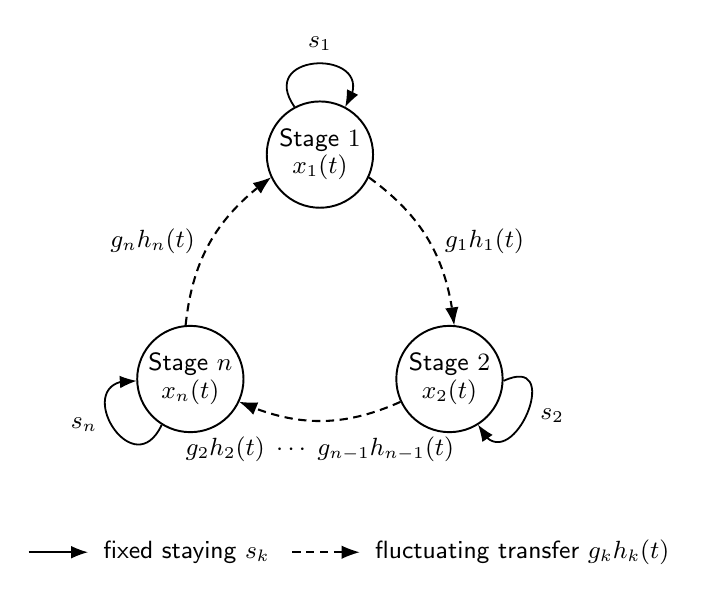
\begin{tikzpicture}[
    font=\sffamily\fontsize{8.5}{10}\selectfont,
    >={Latex[line width=0pt]},
    stage/.style={
        circle,
        draw=black,
        line width=0.7pt,
        minimum size=13.5mm,
        inner sep=1pt,
        align=center,
        fill=white
    },
    stay/.style={
        ->,
        draw=black,
        line width=0.65pt
    },
    fluct/.style={
        ->,
        draw=black,
        line width=0.75pt,
         densely dashed
    }
]

% Bounding width ~82mm so 84mm inclusion is ~1:1 scale
\node[stage] (S1) at (90:19mm) {Stage $1$\\[-1pt]$x_1(t)$};
\node[stage] (S2) at (330:19mm) {Stage $2$\\[-1pt]$x_2(t)$};
\node[stage] (Sn) at (210:19mm) {Stage $n$\\[-1pt]$x_n(t)$};

% Fixed staying self-loops (solid)
\draw[stay] (S1.118) .. controls +(125:9mm) and +(55:9mm) ..
    node[above=1pt] {$s_1$} (S1.62);
\draw[stay] (S2.358) .. controls +(25:9mm) and +(295:9mm) ..
    node[right=1.5pt] {$s_2$} (S2.302);
\draw[stay] (Sn.238) .. controls +(245:9mm) and +(175:9mm) ..
    node[left=1.5pt] {$s_n$} (Sn.182);

% Fluctuating host-driven transfers (dashed)
\draw[fluct] (S1.335) to[bend left=24]
    node[midway, right=2pt, align=left] {$g_1 h_1(t)$} (S2.85);
\draw[fluct] (S2.205) to[bend left=24]
    node[midway, below=2pt, align=center] {$g_2 h_2(t)\;\cdots\;g_{n-1}h_{n-1}(t)$} (Sn.335);
\draw[fluct] (Sn.95) to[bend left=24]
    node[midway, left=2pt, align=right] {$g_n h_n(t)$} (S1.205);

% Compact legend at bottom for line styles
\coordinate (L0) at (-37mm,-31.5mm);
\draw[stay] (L0) -- ++(7.5mm,0) node[right=2pt, anchor=west] {fixed staying $s_k$};
\draw[fluct] ($(L0)+(33.5mm,0)$) -- ++(8.5mm,0) node[right=2pt, anchor=west] {fluctuating transfer $g_k h_k(t)$};

\end{tikzpicture}
\end{jmbfigure}
\end{document}
